%%%%%%%%%%%%%%%%%%%%%%%%%%%%%%%%%%%%%%%%%%%%%%%%%%%%%%%%%%%%%%%%%%%%%%%%%
%%%% Plantilla realizada por César Martínez cesar.martinez@udlap.mx %%%%%
%%%%%%%%%%%%%%%%%%%%%%%%%%%%VERSION 1.0%%%%%%%%%%%%%%%%%%%%%%%%%%%%%%%%%%
%%%%%%%%%%%%%%%%%%%%%%%%%%%%%%%%%%%%%%%%%%%%%%%%%%%%%%%%%%%%%%%%%%%%%%%%%
%%%%%%%%%%%%%%%%%%%%%%%%%%%%%%%%%%%%%%%%%%%%%%%%%%%%%%%%%%%%%%%%%%%%%%%%%


\documentclass[12pt]{article}  %tipo de documento y tamaño de letra normal
%%%%%%%%%%%%%%%%%%%%%%%%%%%%%%%%%%%%%%%%%%%%%%%%%%%%%%%%%%%%%%%%%%%%%
%%%%%%%%%%%%%%%%%%%%%%%%%%%%%%%%%%%%%%%%%%%%%%%%%%%%%%%%%%%%%%%%%%%%%
%%%%%%%%%%%%%%%%%%%%%%%%%%%%%%%%%%%%%%%%%%%%%%%%%%%%%%%%%%%%%%%%%%%%%
%%%%%%%% Paquetes basicos, pueden encontrar información especifica de cada uno de ellos en  (https://www.ctan.org/) %%%%%%%%%%%%%%%%%%%%%%% %%%%%%%%%%%%%%%%%%%%%%%%%%%%%%%%%%%%%%%%%%%%%%%%%%%%%%%%%%%%%%%%%%%%%
%%%%%%%%%%%%%%%%%%%%%%%%%%%%%%%%%%%%%%%%%%%%%%%%%%%%%%%%%%%%%%%%%%%%%
%%%%%%%%%%%%%%%%%%%%%%%%%%%%%%%%%%%%%%%%%%%%%%%%%%%%%%%%%%%%%%%%%%%%%
%\usepackage[spanish]{babel} %Indica que escribiermos en español
\usepackage[english]{babel} %Indica que escribiermos en inglés
%Comentar la línea del idioma que NO usarán en su reporte
\usepackage[utf8]{inputenc} %Indica qué codificación se está usando ISO-8859-1(latin1)  o utf8  
\usepackage{amsmath} % Comandos extras para matemáticas (cajas para ecuaciones,etc)
\usepackage{amssymb} % Simbolos matematicos (por lo tanto)
\usepackage{graphicx} % Incluir imágenes en LaTeX
\usepackage{color} % Para colorear texto
\usepackage{subfigure} % subfiguras
\usepackage{enumerate} % enumerar
\usepackage{commath} % funcionalidades extras para diferenciales, integrales,etc (\od, \dif, etc)
\usepackage{cancel} % para cancelar expresiones (\cancelto{0}{x})
\usepackage{float} %Podemos usar el especificador [H] en las figuras para que se queden donde queramos
\usepackage{appendix} %Para crear apendices
\usepackage{xcolor} %Definir colores personalizados
%%%%%%%%%%%%%%%%%%%%%%%%%%%%%%%%%%%%%%%%%%%%%%%%%%%%%%%%%%%%%%%%%%%%%
%%%%%%%%% PAQUETES CON OPCIONES ESPECIFICAS PRECARGADAS %%%%%%%%%%%%%
%%%%%%%%%%%%%%%%%%%%%%%%%%%%%%%%%%%%%%%%%%%%%%%%%%%%%%%%%%%%%%%%%%%%%
%%%%%%%%%%%%% Permitir agregar código, colocarlo en un rectángulo y  numerarlo %%%%%%%%%%%%%%%%%%%%%%%%%%%%%%%%%%%%%%%%%%%%%%%%%%%%%%%%%%%
%%%%%%%%%%%%%%%%%%%%%%%%%%%%%%%%%%%%%%%%%%%%%%%%%%%%%%%%%%%%%%%%%%%%%
%%%%%%%%%%%%%%%%%%%%%%%%%%%%%%%%%%%%%%%%%%%%%%%%%%%%%%%%%%%%%%%%%%%%%%%%%%%%%%%%%%%%%%%%%%%%%%%%%%%%%%%%%%%%%%%%%%%%%%%%%%%%%%%%%%%%%%%%%%
\usepackage{listings} %Sirve para pegar codigo fuente de programas
\usepackage{caption} %Agregar titulos a los codigos
\DeclareCaptionFont{white}{\color{white}}
\DeclareCaptionFormat{listing}{%
  \parbox{\textwidth}{\colorbox{gray}{\parbox{\textwidth}{#1#2#3}}\vskip-4pt}}
\captionsetup[lstlisting]{format=listing,labelfont=white,textfont=white}
\lstset{frame=lrb,xleftmargin=\fboxsep,xrightmargin=-\fboxsep}
\renewcommand{\lstlistingname}{Código}
%%%%%%%%%%%%%%%%%%%%%%%%%%%%%%%%%%%%%%%%%%%%%%%%%%%%%%%%%%%%%%%%%%%%%
%%% Definir márgenes del documento%%%%%%%%%%%%%%%%%%%%%%%%%%%%%%%%%%%
%%%%%%%%%%%%%%%%%%%%%%%%%%%%%%%%%%%%%%%%%%%%%%%%%%%%%%%%%%%%%%%%%%%%%
 \usepackage{anysize} % Para personalizar el ancho de  los márgenes
\marginsize{2cm}{2cm}{2cm}{2cm} % Izquierda, derecha, arriba, abajo
%%%%%%%%%%%%%%%%%%%%%%%%%%%%%%%%%%%%%%%%%%%%%%%%%%%%%%%%%%%%%%%%%%%%
%%% Hipervinculos activos y a color %%%%%%%%%%%%%%%%%%%%%%%%%%%%%%%%
%%%%%%%%%%%%%%%%%%%%%%%%%%%%%%%%%%%%%%%%%%%%%%%%%%%%%%%%%%%%%%%%%%%%%
\usepackage[colorlinks=true,plainpages=true,citecolor=blue,linkcolor=black]{hyperref}
\usepackage{hyperref} 
%%%%%%%%%%%%%%%%%%%%%%%%%%%%%%%%%%%%%%%%%%%%%%%%%%%%%%%%%%%%%%%%%%%%%
%%%%%% Encabezado y pie de pagina %%%%%%%%%%%%%%%%%%%%%%%%%%%%%%%%%%%
%%%%%%%%%%%%%%%%%%%%%%%%%%%%%%%%%%%%%%%%%%%%%%%%%%%%%%%%%%%%%%%%%%%%%
\usepackage{fancyhdr} 
\pagestyle{fancy}
\fancyhf{}
\fancyhead[L]{\footnotesize UDLAP} %encabezado izquierda
\fancyhead[R]{\footnotesize CEM}   % encabezado derecha
\fancyfoot[R]{\footnotesize \curso}  % Pie derecha
\fancyfoot[C]{\thepage}  % centro
\fancyfoot[L]{}  %izquierda
\renewcommand{\footrulewidth}{0.4pt}
%%%%%%%%%%%%%%%%%%%%%%%%%%%%%%%%%%%%%%%%%%%%%%%%%%%%%%%%%%%%%%%%%%%%%
%%%% Carpeta donde se deben colocar las imagenes %%%%%%%%%%%%%%%%%%%%
\graphicspath{{Imagenes/}} %Colocar aqui todas las imagenes del documento pueden estar en formato png, eps o jpg, se recomienda eps para mayor calidad.
%%%%%%%%%%%%%%%%%%%%%%%%%%%%%%%%%%%%%%%%%%%%%%%%%%%%%%%%%%%%%%%%%%%%%
%%%%%%%%%%%%%%%%%%%%%%%%%%%%%%%%%%%%%%%%%%%%%%%%%%%%%%%%%%%%%%%%%%%%%
%%%%%%%% Termina carga de paquetes %%%%%%%%%%%%%%%%%%%%%%%%%%%%%%%%%%% 
%%%%%%%%%%%%%%%%%%%%%%%%%%%%%%%%%%%%%%%%%%%%%%%%%%%%%%%%%%%%%%%%%%%%%
%%%%%%%%%%%%%%%%%%%%%%%%%%%%%%%%%%%%%%%%%%%%%%%%%%%%%%%%%%%%%%%%%%%%%
%%%%%%%%%%%%%%%%%%%%%%%%%%%%%%%%%%%%%%%%%%%%%%%%%%%%%%%%%%%%%%%%%%%%%
%%%%%% Modificar campos que aparecerán en portada %%%%%%%%%%%%%%%%%%%
%%%%%%%%%%%%%%%%%%%%%%%%%%%%%%%%%%%%%%%%%%%%%%%%%%%%%%%%%%%%%%%%%%%%%
%%%%%%%%%%%%%%%%%%%%%%%%%%%%%%%%%%%%%%%%%%%%%%%%%%%%%%%%%%%%%%%%%%%%%
%%%%%%%%%%%%%%%%%%%%%%%%%%%%%%%%%%%%%%%%%%%%%%%%%%%%%%%%%%%%%%%%%%%%%
\def\titulo{Lab report \#1}%titulo del documento
\def\materia{Course: Digital design LRT2022-sección} %Clave nombre de la materia y sección
\def\curso{Digital design} %Nombre de la materia para footnote
\def\fecha{April 1st, 20} %En formato mes, dia año
\def\equipo {2}%Verificar en blackboard el número asignado
\def\ida{183339} %Nombre y Id´s de todos los integrantes que hayan trabajado en el proyecto
\def\esta{Juan Pablo Lopez Moreno}
\def\lica{LMT}%LRT,LBM,LIS,LMT
\def\idb{185406}
\def\estb{Amy Marianee Ramírez Sánchez}
\def\licb{LMT}%LRT,LBM,LIS,LMT
%Copiar y pegar más líneas si su equipo tiene más de 5 integrantes, eliminar si está formado por menos
%%%%%%%%%%%%%%%%%%%%%%%%%%%%%%%%%%%%%%%%%%%%%%%%%%%%%%%%%%%%%%%%%%%%%
%%%%%%%%%%%%%%%%%%%%%%%%%%%%%%%%%%%%%%%%%%%%%%%%%%%%%%%%%%%%%%%%%%%%%
%%%%%%%%%%%%%%%%%%%%%%%%%%%%%%%%%%%%%%%%%%%%%%%%%%%%%%%%%%%%%%%%%%%%%
\begin{document} %Inicia el documento
%%%%%%%%%%%%%%%%%%%%%%%%%%%%%%%%%%%%%%%%%%%%%%%%%%%%%%%%%%%%%%%%%%%%%
%%%%%%%%%%%%%%%%%%%%%%%%%%%%%%%%%%%%%%%%%%%%%%%%%%%%%%%%%%%%%%%%%%%%%
%%%%%%%%%%%%%%%%%%%%%%%%%%%%%%%%%%%%%%%%%%%%%%%%%%%%%%%%%%%%%%%%%%%%%
%%%%%%%%%%%%%%%%%%%%%%%%%%%%%%%%%% PORTADA %%%%%%%%%%%%%%%%%%%%%%%%%%
%%%%%%%%%%%%%%%%%%%%%%%%%%%%%%%%%%%%%%%%%%%%%%%%%%%%%%%%%%%%%%%%%%%%%No es necesario modificar ninguna de las siguientes lineas, sólo si el número de estudiantes que conforman su equipo es menor o mayor a 5
%%%%%%%%%%%%%%%%%%%%%%%%%%%%%%%%%%%%%%%%%%%%%%%%%%%%%%%%%%%%%%%%%%%%%
%%%%%%%%%%%%%%%%%%%%%%%%%%%%%%%%%%%%%%%%%%%%%%%%%%%%%%%%%%%%%%%%%%%%%
%%%%%%%%%%%%%%%%%%%%%%%%%%%%%%%%%%%%%%%%%%%%%%%%%%%%%%%%%%%%%%%%%%%%%
\begin{center}														
\newcommand{\HRule}{\rule{\linewidth}{0.5mm}}						
\thispagestyle{empty} 												
\vspace*{-1.5cm}								
\textsc{\huge Universidad de las Américas Puebla}\\[1.5cm]	
\textsc{\LARGE Escuela de ingeniería}\\[1.5cm]	
\textsc{\LARGE Departamento de computación, electrónica y mecatrónica}\\[1.5cm]												
\includegraphics[width=150mm]{UDLAP}  									\vspace*{1cm}														\HRule \\[0.4cm]												
{ \huge \bfseries \titulo}\\[0.4cm]	
\HRule \\[1cm]														
{ \Large \bfseries \materia}\\[1cm] 	
{ \Large \bfseries Equipo: \equipo}\\[1cm] 							
\begin{flushleft} \Large											
\ida \hspace{0.5cm}\esta \hspace{0.5cm} \lica\\
\idb \hspace{0.5cm}\estb \hspace{0.5cm} \licb\\
%Copiar y pegar más líneas si su equipo tiene más de 2 integrantes, eliminar si la entrega es individual
\end{flushleft}														
\vfill																
\begin{center}													
{\Large  \fecha, San Andrés Cholula, Puebla}						
\end{center}												 		
\end{center}							 								\newpage						
%%%%%%%%%%%%%%%%%%%% TERMINA PORTADA %%%%%%%%%%%%%%%%%%%%%%%%%%%%%%%%
%%%%%%%%%%%%%%%%%%%%%%%%%%%%%%%%%%%%%%%%%%%%%%%%%%%%%%%%%%%%%%%%%%%%%
%%%%%%%%%%%%%%%%%%%%%%%%%%%%%%%%%%%%%%%%%%%%%%%%%%%%%%%%%%%%%%%%%%%%%
%%%%%%%%%%%%%%%%%%%%%%%%%%%%%%%%%%%%%%%%%%%%%%%%%%%%%%%%%%%%%%%%%%%%%
%%%%%%%%%%%%%%%%%%%%%%%%%%%%%%%%%%%%%%%%%%%%%%%%%%%%%%%%%%%%%%%%%%%%%
\setcounter{page}{1} %Para comenzar a numerar las páginas desde este punto
\section{Abstract} %Síntesis del reporte en un solo párrafo

\section{Introduction} %Breve introducción al tema del reporte
A fundamental part of working with circuits is to have knowledge about the tools that will be used during the design of these components.

During the course of Digital Design, it will be elemental to have a knowledge of the inner workings of certain electronics, 
especially to find a way to showcase the values resulting from logical operations. Considering the previous statement, during the first and second day of lab work, 
the team will focus on understanding and employing simple circuits that will help to understand the basic concepts of digital electronics. 
The main tools that will be used during this lab are the multimeter and the power supply, showcasing their usage through circuits developed both in a breadboard and in Multisim.
\section{Objectives} %Objetivos de la práctica
The objectives of this lab are:
\begin{itemize}
  \item Learn to use the Multimeter and the power supply.
  \item Implement a circuit of digital input and output in a breadboard and Multisim.
  \item Verify the proper functioning of the digital circuits by using the Multimeter.
\end{itemize}
A multimeter is defined as an instrument that measures different electrical quantities such as current, voltage, and resistance, and can be either analogue or digital. It is used for tasks like fault finding and assessing the condition of electrical components, with digital meters offering greater accuracy and ease of reading. \cite{SDMultimeter}
\\A power supply is defined as the interface between an external power source, which may be noisy and variable, and the clear-cut requirements of internal circuitry in electronic products. It typically takes power from a conventional AC mains supply, though other options like low-voltage DC or specific aircraft supplies may also be used. \cite{SDPowerSupply}

\section{Methodology} %Desarrollo de la práctica

\section{Results} %Resultados obtenidos
\subsection{Digital lab experimentation}
During the lab, the team was able to obtain these results from the experimentation in both the breadboard and Multisim. The results are precented as follows:
For the first part, the team developed the simulation of the circuit 1 and 2 in Multisim, obtaining the following diagrams:
\begin{figure}[H]
    \centering
    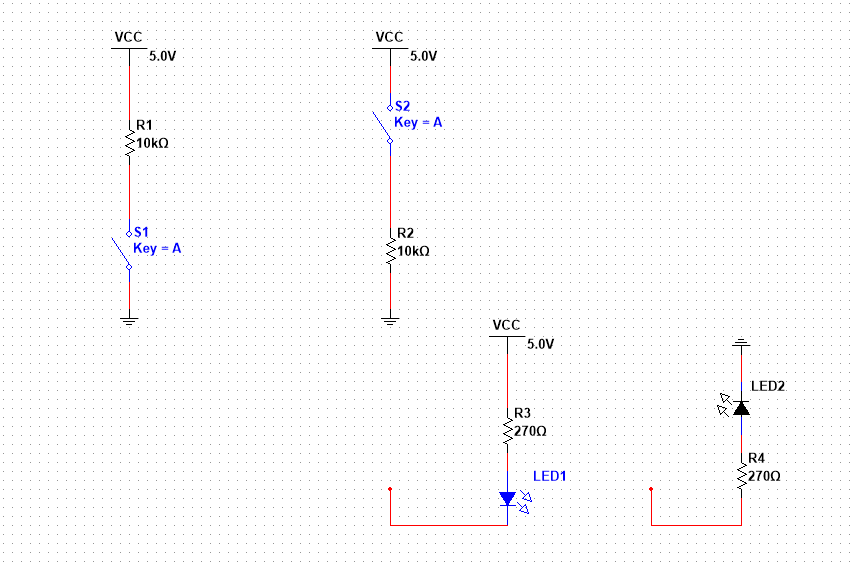
\includegraphics[width=0.7\textwidth]{Circuit 1 and 2.png}
    \caption{Circuits developed in Multisim}
    \label{fig:multisim_circuits}
\end{figure}
After the development of the circuits, the team was able to measure the voltage in the output of both circuits. Obtaining this values based on the measurement of the circuits in Multisim:
\begin{figure}[H]
    \centering
    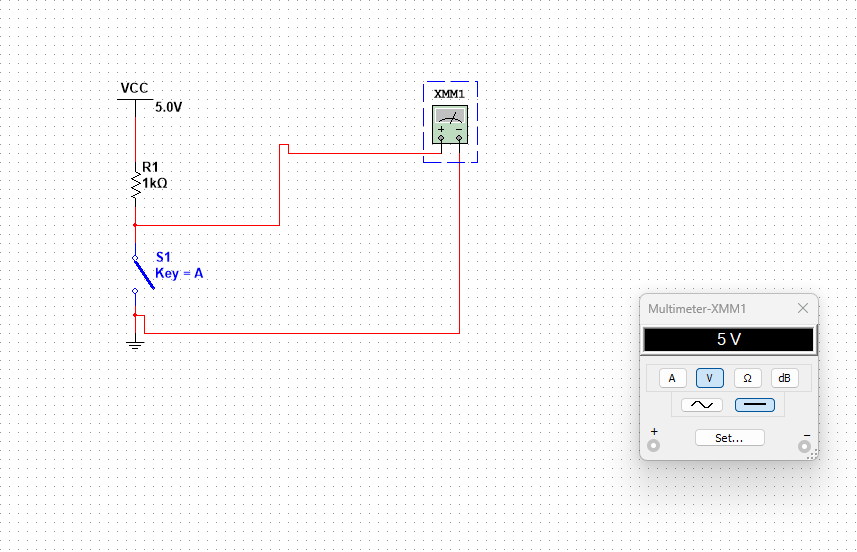
\includegraphics[scale=0.3]{Prueba1.png}
    \hfill
    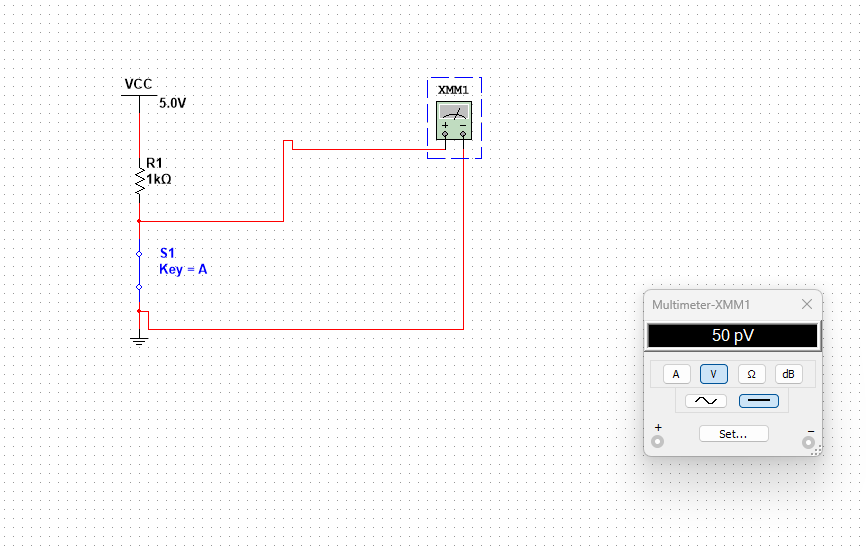
\includegraphics[scale=0.3]{Prueba2.png}
    \caption{Circuits developed in Multisim}
    \label{fig:multisim_circuits_measurements}
\end{figure}
\subsection{Physical lab experimentation}
For the physical lab, the team developed the same circuits in a breadboard, obtaining the following circuits:
\begin{figure}[H]
  \centering
  \begin{minipage}{0.25\textwidth}
    \centering
    \includegraphics[width=\textwidth]{Circuito 1.png}
  \end{minipage}
  \hspace{0.05\textwidth}
  \begin{minipage}{0.25\textwidth}
    \centering
    \includegraphics[width=\textwidth]{Circuito 2.png}
  \end{minipage}
  \caption{Circuits developed in breadboard}
  \label{fig:breadboard_circuits}
\end{figure}
These measurements were taken to ensure that the results were as expected.

\begin{figure}[H]
  \centering
  \begin{minipage}{0.25\textwidth}
    \centering
    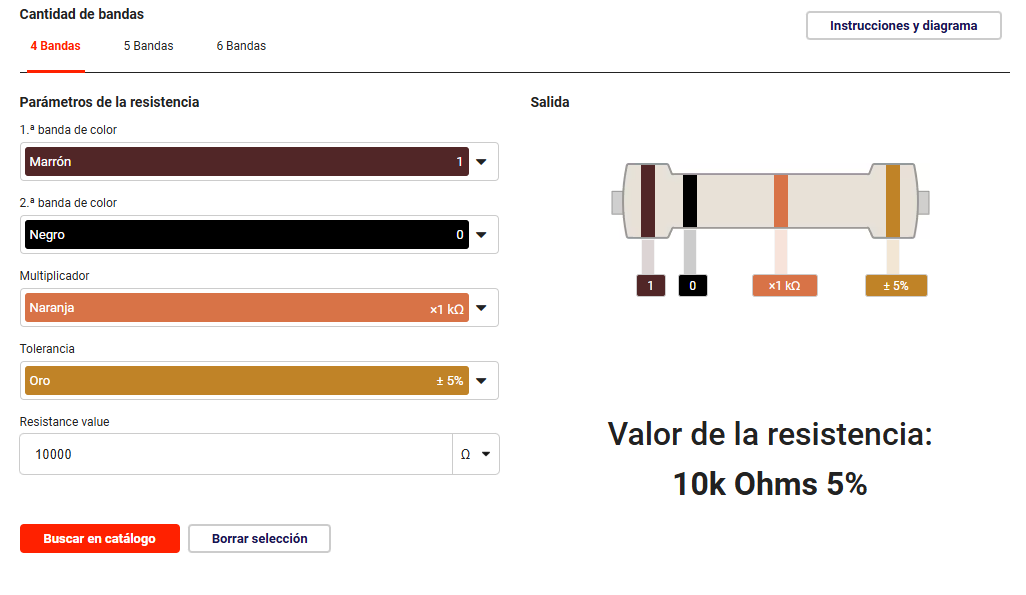
\includegraphics[width=\textwidth]{Resistencia1.png}
  \end{minipage}
  \hspace{0.05\textwidth}
  \begin{minipage}{0.25\textwidth}
    \centering
    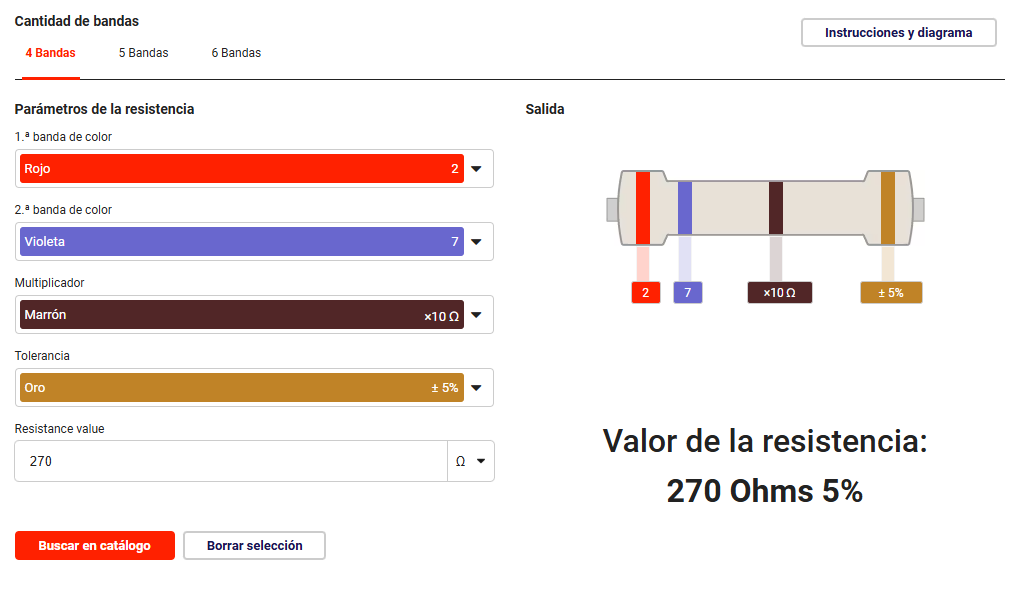
\includegraphics[width=\textwidth]{Resistencia2.png}
  \end{minipage}
  \begin{minipage}{0.25\textwidth}
    \centering
    \includegraphics[width=\textwidth]{MedidaCircuito.png}
  \end{minipage}
  \caption{Measurements taken in breadboard circuits}
  \label{fig:breadboard_measurement}
\end{figure}

Finally, in order to have a correct method for testing the functionality of logic gates in the future, the circuit functionality was turned into a table for easy understanding.

For the first circuit, the following table was made:
\begin{table}[H]
  \centering
  \begin{tabular}{|l|c|c|}
    \hline
    \textbf{Switch status} & \textbf{Voltage measured} & \textbf{Logic state} \\
    \hline
    On & 0 & Low \\
    Off & 4.99 & High \\
    \hline
  \end{tabular}
  \caption{Pull-up Resistor}
  \label{tab:pullup}
\end{table}

For the second circuit, the following table was made:
\begin{table}[H]
  \centering
  \begin{tabular}{|l|c|c|}
    \hline
    \textbf{Switch status} & \textbf{Voltage measured} & \textbf{Logic state} \\
    \hline
    On & 5.00 & High \\
    Off & 0 & Low \\
    \hline
  \end{tabular}
  \caption{Pull-down Resistor}
  \label{tab:pulldown}
\end{table}

For the third circuit, the following table was made:
\begin{table}[H]
  \centering
  \begin{tabular}{|l|c|c|}
    \hline
    \textbf{Output logic state} & \textbf{Voltage measured} & \textbf{LED status} \\
    \hline
    High & 0 & Off \\
    Low & 4.99 & On \\
    \hline
  \end{tabular}
  \caption{Active Low}
  \label{tab:activelow}
\end{table}

Finally, for the fourth circuit, the following table was made:
\begin{table}[H]
  \centering
  \begin{tabular}{|l|c|c|}
    \hline
    \textbf{Output logic state} & \textbf{Voltage measured} & \textbf{LED status} \\
    \hline
    High & 4.99 & On \\
    Low & 0 & Off \\
    \hline
  \end{tabular}
  \caption{Active High}
  \label{tab:activehigh}
\end{table}
\section{Analysis} %Análisis de los resultados obtenidos
\section{Conclusions} %Conclusiones del reporte
%%%%%%% Bibliografía %%%%%%%%
\clearpage %Asegura que la bibliografía inicie en una nueva página
\bibliographystyle{bst/IEEEtran} %Estilo de bibliografía NO MODIFICAR PARA MANTENER FORMATO
\bibliography{bib/bibliografia} %Fuentes bibliográficas Se recomienda utilizar un gestor de referencias (zotero, jabref, etc..)
%%%%%%% Bibliografía %%%%%%%%      
\end{document} %Termina el documento
%% Known issues and TODO list%%%
% Warning overfull \hbox en los códigos
% Código en texto blanco y negro y comentarios en negritas => Cambiar a formato en colores